\section{Organisationsplan för hela projektet}
Beställaren har beställt projektet från gruppen. Analysansvarig är den medlem i gruppen som agerar mellanhand mellan projektgruppen och beställaren. Varje medlem i projektgruppen har ett ansvarsområde där han eller hon leder en arbetsgrupp bestående av delar av resten av gruppen. Det innebär att varje medlem är både arbetsledare och del i minst ett annat arbetslag. En handledare finns tillgänglig för att hjälpa gruppen på vägen. Figur \ref{projektplan:organisationsplan} illustrerar strukturen.

\begin{figure}[H]
\center
\tikzset{every picture/.style={scale=0.6}}%
% Graphic for TeX using PGF
% Title: /home/kebabdjuret/Documents/skola/tddd77/repo/dokumentation/projektplan/grafik/projektplan-organisationsplan.dia
% Creator: Dia v0.97.2
% CreationDate: Fri Feb 13 14:31:28 2015
% For: kebabdjuret
% \usepackage{tikz}
% The following commands are not supported in PSTricks at present
% We define them conditionally, so when they are implemented,
% this pgf file will use them.
\ifx\du\undefined
  \newlength{\du}
\fi
\setlength{\du}{15\unitlength}
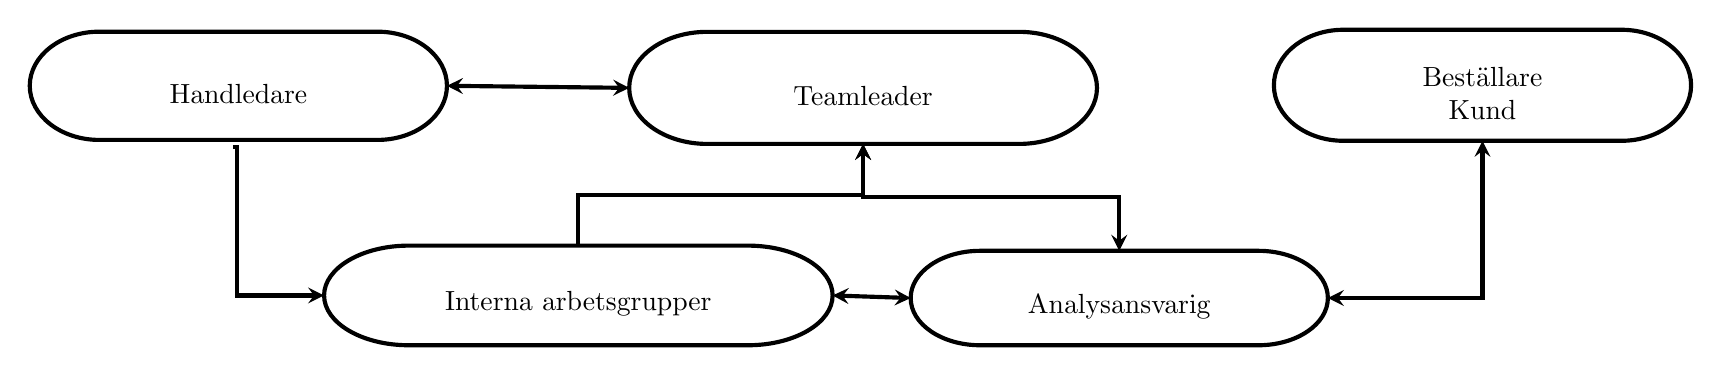
\begin{tikzpicture}
\pgftransformxscale{1.000000}
\pgftransformyscale{-1.000000}
\definecolor{dialinecolor}{rgb}{0.000000, 0.000000, 0.000000}
\pgfsetstrokecolor{dialinecolor}
\definecolor{dialinecolor}{rgb}{1.000000, 1.000000, 1.000000}
\pgfsetfillcolor{dialinecolor}
\pgfsetlinewidth{0.100000\du}
\pgfsetdash{}{0pt}
\pgfsetdash{}{0pt}
\pgfsetbuttcap
\pgfsetmiterjoin
\pgfsetlinewidth{0.100000\du}
\pgfsetbuttcap
\pgfsetmiterjoin
\pgfsetdash{}{0pt}
\definecolor{dialinecolor}{rgb}{1.000000, 1.000000, 1.000000}
\pgfsetfillcolor{dialinecolor}
\pgfpathmoveto{\pgfpoint{37.805600\du}{22.350000\du}}
\pgfpathlineto{\pgfpoint{44.505600\du}{22.350000\du}}
\pgfpathcurveto{\pgfpoint{45.430677\du}{22.350000\du}}{\pgfpoint{46.180600\du}{22.948819\du}}{\pgfpoint{46.180600\du}{23.687500\du}}
\pgfpathcurveto{\pgfpoint{46.180600\du}{24.426181\du}}{\pgfpoint{45.430677\du}{25.025000\du}}{\pgfpoint{44.505600\du}{25.025000\du}}
\pgfpathlineto{\pgfpoint{37.805600\du}{25.025000\du}}
\pgfpathcurveto{\pgfpoint{36.880523\du}{25.025000\du}}{\pgfpoint{36.130600\du}{24.426181\du}}{\pgfpoint{36.130600\du}{23.687500\du}}
\pgfpathcurveto{\pgfpoint{36.130600\du}{22.948819\du}}{\pgfpoint{36.880523\du}{22.350000\du}}{\pgfpoint{37.805600\du}{22.350000\du}}
\pgfusepath{fill}
\definecolor{dialinecolor}{rgb}{0.000000, 0.000000, 0.000000}
\pgfsetstrokecolor{dialinecolor}
\pgfpathmoveto{\pgfpoint{37.805600\du}{22.350000\du}}
\pgfpathlineto{\pgfpoint{44.505600\du}{22.350000\du}}
\pgfpathcurveto{\pgfpoint{45.430677\du}{22.350000\du}}{\pgfpoint{46.180600\du}{22.948819\du}}{\pgfpoint{46.180600\du}{23.687500\du}}
\pgfpathcurveto{\pgfpoint{46.180600\du}{24.426181\du}}{\pgfpoint{45.430677\du}{25.025000\du}}{\pgfpoint{44.505600\du}{25.025000\du}}
\pgfpathlineto{\pgfpoint{37.805600\du}{25.025000\du}}
\pgfpathcurveto{\pgfpoint{36.880523\du}{25.025000\du}}{\pgfpoint{36.130600\du}{24.426181\du}}{\pgfpoint{36.130600\du}{23.687500\du}}
\pgfpathcurveto{\pgfpoint{36.130600\du}{22.948819\du}}{\pgfpoint{36.880523\du}{22.350000\du}}{\pgfpoint{37.805600\du}{22.350000\du}}
\pgfusepath{stroke}
% setfont left to latex
\definecolor{dialinecolor}{rgb}{0.000000, 0.000000, 0.000000}
\pgfsetstrokecolor{dialinecolor}
\node at (41.155600\du,23.487500\du){Beställare};
% setfont left to latex
\definecolor{dialinecolor}{rgb}{0.000000, 0.000000, 0.000000}
\pgfsetstrokecolor{dialinecolor}
\node at (41.155600\du,24.287500\du){Kund};
\pgfsetlinewidth{0.100000\du}
\pgfsetdash{}{0pt}
\pgfsetdash{}{0pt}
\pgfsetbuttcap
\pgfsetmiterjoin
\pgfsetlinewidth{0.100000\du}
\pgfsetbuttcap
\pgfsetmiterjoin
\pgfsetdash{}{0pt}
\definecolor{dialinecolor}{rgb}{1.000000, 1.000000, 1.000000}
\pgfsetfillcolor{dialinecolor}
\pgfpathmoveto{\pgfpoint{22.478125\du}{22.400000\du}}
\pgfpathlineto{\pgfpoint{29.990625\du}{22.400000\du}}
\pgfpathcurveto{\pgfpoint{31.027885\du}{22.400000\du}}{\pgfpoint{31.868750\du}{23.004415\du}}{\pgfpoint{31.868750\du}{23.750000\du}}
\pgfpathcurveto{\pgfpoint{31.868750\du}{24.495585\du}}{\pgfpoint{31.027885\du}{25.100000\du}}{\pgfpoint{29.990625\du}{25.100000\du}}
\pgfpathlineto{\pgfpoint{22.478125\du}{25.100000\du}}
\pgfpathcurveto{\pgfpoint{21.440865\du}{25.100000\du}}{\pgfpoint{20.600000\du}{24.495585\du}}{\pgfpoint{20.600000\du}{23.750000\du}}
\pgfpathcurveto{\pgfpoint{20.600000\du}{23.004415\du}}{\pgfpoint{21.440865\du}{22.400000\du}}{\pgfpoint{22.478125\du}{22.400000\du}}
\pgfusepath{fill}
\definecolor{dialinecolor}{rgb}{0.000000, 0.000000, 0.000000}
\pgfsetstrokecolor{dialinecolor}
\pgfpathmoveto{\pgfpoint{22.478125\du}{22.400000\du}}
\pgfpathlineto{\pgfpoint{29.990625\du}{22.400000\du}}
\pgfpathcurveto{\pgfpoint{31.027885\du}{22.400000\du}}{\pgfpoint{31.868750\du}{23.004415\du}}{\pgfpoint{31.868750\du}{23.750000\du}}
\pgfpathcurveto{\pgfpoint{31.868750\du}{24.495585\du}}{\pgfpoint{31.027885\du}{25.100000\du}}{\pgfpoint{29.990625\du}{25.100000\du}}
\pgfpathlineto{\pgfpoint{22.478125\du}{25.100000\du}}
\pgfpathcurveto{\pgfpoint{21.440865\du}{25.100000\du}}{\pgfpoint{20.600000\du}{24.495585\du}}{\pgfpoint{20.600000\du}{23.750000\du}}
\pgfpathcurveto{\pgfpoint{20.600000\du}{23.004415\du}}{\pgfpoint{21.440865\du}{22.400000\du}}{\pgfpoint{22.478125\du}{22.400000\du}}
\pgfusepath{stroke}
% setfont left to latex
\definecolor{dialinecolor}{rgb}{0.000000, 0.000000, 0.000000}
\pgfsetstrokecolor{dialinecolor}
\node at (26.234375\du,23.950000\du){Teamleader};
\pgfsetlinewidth{0.100000\du}
\pgfsetdash{}{0pt}
\pgfsetdash{}{0pt}
\pgfsetbuttcap
\pgfsetmiterjoin
\pgfsetlinewidth{0.100000\du}
\pgfsetbuttcap
\pgfsetmiterjoin
\pgfsetdash{}{0pt}
\definecolor{dialinecolor}{rgb}{1.000000, 1.000000, 1.000000}
\pgfsetfillcolor{dialinecolor}
\pgfpathmoveto{\pgfpoint{7.834370\du}{22.396200\du}}
\pgfpathlineto{\pgfpoint{14.534370\du}{22.396200\du}}
\pgfpathcurveto{\pgfpoint{15.459447\du}{22.396200\du}}{\pgfpoint{16.209370\du}{22.979908\du}}{\pgfpoint{16.209370\du}{23.699950\du}}
\pgfpathcurveto{\pgfpoint{16.209370\du}{24.419992\du}}{\pgfpoint{15.459447\du}{25.003700\du}}{\pgfpoint{14.534370\du}{25.003700\du}}
\pgfpathlineto{\pgfpoint{7.834370\du}{25.003700\du}}
\pgfpathcurveto{\pgfpoint{6.909293\du}{25.003700\du}}{\pgfpoint{6.159370\du}{24.419992\du}}{\pgfpoint{6.159370\du}{23.699950\du}}
\pgfpathcurveto{\pgfpoint{6.159370\du}{22.979908\du}}{\pgfpoint{6.909293\du}{22.396200\du}}{\pgfpoint{7.834370\du}{22.396200\du}}
\pgfusepath{fill}
\definecolor{dialinecolor}{rgb}{0.000000, 0.000000, 0.000000}
\pgfsetstrokecolor{dialinecolor}
\pgfpathmoveto{\pgfpoint{7.834370\du}{22.396200\du}}
\pgfpathlineto{\pgfpoint{14.534370\du}{22.396200\du}}
\pgfpathcurveto{\pgfpoint{15.459447\du}{22.396200\du}}{\pgfpoint{16.209370\du}{22.979908\du}}{\pgfpoint{16.209370\du}{23.699950\du}}
\pgfpathcurveto{\pgfpoint{16.209370\du}{24.419992\du}}{\pgfpoint{15.459447\du}{25.003700\du}}{\pgfpoint{14.534370\du}{25.003700\du}}
\pgfpathlineto{\pgfpoint{7.834370\du}{25.003700\du}}
\pgfpathcurveto{\pgfpoint{6.909293\du}{25.003700\du}}{\pgfpoint{6.159370\du}{24.419992\du}}{\pgfpoint{6.159370\du}{23.699950\du}}
\pgfpathcurveto{\pgfpoint{6.159370\du}{22.979908\du}}{\pgfpoint{6.909293\du}{22.396200\du}}{\pgfpoint{7.834370\du}{22.396200\du}}
\pgfusepath{stroke}
% setfont left to latex
\definecolor{dialinecolor}{rgb}{0.000000, 0.000000, 0.000000}
\pgfsetstrokecolor{dialinecolor}
\node at (11.184370\du,23.899950\du){Handledare};
\pgfsetlinewidth{0.100000\du}
\pgfsetdash{}{0pt}
\pgfsetdash{}{0pt}
\pgfsetbuttcap
\pgfsetmiterjoin
\pgfsetlinewidth{0.100000\du}
\pgfsetbuttcap
\pgfsetmiterjoin
\pgfsetdash{}{0pt}
\definecolor{dialinecolor}{rgb}{1.000000, 1.000000, 1.000000}
\pgfsetfillcolor{dialinecolor}
\pgfpathmoveto{\pgfpoint{29.055600\du}{27.675000\du}}
\pgfpathlineto{\pgfpoint{35.755600\du}{27.675000\du}}
\pgfpathcurveto{\pgfpoint{36.680677\du}{27.675000\du}}{\pgfpoint{37.430600\du}{28.184276\du}}{\pgfpoint{37.430600\du}{28.812500\du}}
\pgfpathcurveto{\pgfpoint{37.430600\du}{29.440724\du}}{\pgfpoint{36.680677\du}{29.950000\du}}{\pgfpoint{35.755600\du}{29.950000\du}}
\pgfpathlineto{\pgfpoint{29.055600\du}{29.950000\du}}
\pgfpathcurveto{\pgfpoint{28.130523\du}{29.950000\du}}{\pgfpoint{27.380600\du}{29.440724\du}}{\pgfpoint{27.380600\du}{28.812500\du}}
\pgfpathcurveto{\pgfpoint{27.380600\du}{28.184276\du}}{\pgfpoint{28.130523\du}{27.675000\du}}{\pgfpoint{29.055600\du}{27.675000\du}}
\pgfusepath{fill}
\definecolor{dialinecolor}{rgb}{0.000000, 0.000000, 0.000000}
\pgfsetstrokecolor{dialinecolor}
\pgfpathmoveto{\pgfpoint{29.055600\du}{27.675000\du}}
\pgfpathlineto{\pgfpoint{35.755600\du}{27.675000\du}}
\pgfpathcurveto{\pgfpoint{36.680677\du}{27.675000\du}}{\pgfpoint{37.430600\du}{28.184276\du}}{\pgfpoint{37.430600\du}{28.812500\du}}
\pgfpathcurveto{\pgfpoint{37.430600\du}{29.440724\du}}{\pgfpoint{36.680677\du}{29.950000\du}}{\pgfpoint{35.755600\du}{29.950000\du}}
\pgfpathlineto{\pgfpoint{29.055600\du}{29.950000\du}}
\pgfpathcurveto{\pgfpoint{28.130523\du}{29.950000\du}}{\pgfpoint{27.380600\du}{29.440724\du}}{\pgfpoint{27.380600\du}{28.812500\du}}
\pgfpathcurveto{\pgfpoint{27.380600\du}{28.184276\du}}{\pgfpoint{28.130523\du}{27.675000\du}}{\pgfpoint{29.055600\du}{27.675000\du}}
\pgfusepath{stroke}
% setfont left to latex
\definecolor{dialinecolor}{rgb}{0.000000, 0.000000, 0.000000}
\pgfsetstrokecolor{dialinecolor}
\node at (32.405600\du,29.012500\du){Analysansvarig};
\pgfsetlinewidth{0.100000\du}
\pgfsetdash{}{0pt}
\pgfsetdash{}{0pt}
\pgfsetbuttcap
\pgfsetmiterjoin
\pgfsetlinewidth{0.100000\du}
\pgfsetbuttcap
\pgfsetmiterjoin
\pgfsetdash{}{0pt}
\definecolor{dialinecolor}{rgb}{1.000000, 1.000000, 1.000000}
\pgfsetfillcolor{dialinecolor}
\pgfpathmoveto{\pgfpoint{15.291667\du}{27.550000\du}}
\pgfpathlineto{\pgfpoint{23.458333\du}{27.550000\du}}
\pgfpathcurveto{\pgfpoint{24.585915\du}{27.550000\du}}{\pgfpoint{25.500000\du}{28.087258\du}}{\pgfpoint{25.500000\du}{28.750000\du}}
\pgfpathcurveto{\pgfpoint{25.500000\du}{29.412742\du}}{\pgfpoint{24.585915\du}{29.950000\du}}{\pgfpoint{23.458333\du}{29.950000\du}}
\pgfpathlineto{\pgfpoint{15.291667\du}{29.950000\du}}
\pgfpathcurveto{\pgfpoint{14.164085\du}{29.950000\du}}{\pgfpoint{13.250000\du}{29.412742\du}}{\pgfpoint{13.250000\du}{28.750000\du}}
\pgfpathcurveto{\pgfpoint{13.250000\du}{28.087258\du}}{\pgfpoint{14.164085\du}{27.550000\du}}{\pgfpoint{15.291667\du}{27.550000\du}}
\pgfusepath{fill}
\definecolor{dialinecolor}{rgb}{0.000000, 0.000000, 0.000000}
\pgfsetstrokecolor{dialinecolor}
\pgfpathmoveto{\pgfpoint{15.291667\du}{27.550000\du}}
\pgfpathlineto{\pgfpoint{23.458333\du}{27.550000\du}}
\pgfpathcurveto{\pgfpoint{24.585915\du}{27.550000\du}}{\pgfpoint{25.500000\du}{28.087258\du}}{\pgfpoint{25.500000\du}{28.750000\du}}
\pgfpathcurveto{\pgfpoint{25.500000\du}{29.412742\du}}{\pgfpoint{24.585915\du}{29.950000\du}}{\pgfpoint{23.458333\du}{29.950000\du}}
\pgfpathlineto{\pgfpoint{15.291667\du}{29.950000\du}}
\pgfpathcurveto{\pgfpoint{14.164085\du}{29.950000\du}}{\pgfpoint{13.250000\du}{29.412742\du}}{\pgfpoint{13.250000\du}{28.750000\du}}
\pgfpathcurveto{\pgfpoint{13.250000\du}{28.087258\du}}{\pgfpoint{14.164085\du}{27.550000\du}}{\pgfpoint{15.291667\du}{27.550000\du}}
\pgfusepath{stroke}
% setfont left to latex
\definecolor{dialinecolor}{rgb}{0.000000, 0.000000, 0.000000}
\pgfsetstrokecolor{dialinecolor}
\node at (19.375000\du,28.950000\du){Interna arbetsgrupper};
% setfont left to latex
\definecolor{dialinecolor}{rgb}{0.000000, 0.000000, 0.000000}
\pgfsetstrokecolor{dialinecolor}
\node[anchor=west] at (26.234375\du,23.750000\du){};
\pgfsetlinewidth{0.100000\du}
\pgfsetdash{}{0pt}
\pgfsetdash{}{0pt}
\pgfsetbuttcap
{
\definecolor{dialinecolor}{rgb}{0.000000, 0.000000, 0.000000}
\pgfsetfillcolor{dialinecolor}
% was here!!!
\pgfsetarrowsstart{stealth}
\pgfsetarrowsend{stealth}
\definecolor{dialinecolor}{rgb}{0.000000, 0.000000, 0.000000}
\pgfsetstrokecolor{dialinecolor}
\draw (20.600000\du,23.750000\du)--(16.209370\du,23.699950\du);
}
\pgfsetlinewidth{0.100000\du}
\pgfsetdash{}{0pt}
\pgfsetdash{}{0pt}
\pgfsetbuttcap
{
\definecolor{dialinecolor}{rgb}{0.000000, 0.000000, 0.000000}
\pgfsetfillcolor{dialinecolor}
% was here!!!
\pgfsetarrowsstart{stealth}
\pgfsetarrowsend{stealth}
\definecolor{dialinecolor}{rgb}{0.000000, 0.000000, 0.000000}
\pgfsetstrokecolor{dialinecolor}
\draw (25.500000\du,28.750000\du)--(27.380600\du,28.812500\du);
}
\pgfsetlinewidth{0.100000\du}
\pgfsetdash{}{0pt}
\pgfsetdash{}{0pt}
\pgfsetmiterjoin
\pgfsetbuttcap
{
\definecolor{dialinecolor}{rgb}{0.000000, 0.000000, 0.000000}
\pgfsetfillcolor{dialinecolor}
% was here!!!
\pgfsetarrowsend{stealth}
{\pgfsetcornersarced{\pgfpoint{0.000000\du}{0.000000\du}}\definecolor{dialinecolor}{rgb}{0.000000, 0.000000, 0.000000}
\pgfsetstrokecolor{dialinecolor}
\draw (11.050000\du,25.175000\du)--(11.150000\du,25.175000\du)--(11.150000\du,28.750000\du)--(13.250000\du,28.750000\du);
}}
\pgfsetlinewidth{0.100000\du}
\pgfsetdash{}{0pt}
\pgfsetdash{}{0pt}
\pgfsetmiterjoin
\pgfsetbuttcap
{
\definecolor{dialinecolor}{rgb}{0.000000, 0.000000, 0.000000}
\pgfsetfillcolor{dialinecolor}
% was here!!!
\pgfsetarrowsend{stealth}
{\pgfsetcornersarced{\pgfpoint{0.000000\du}{0.000000\du}}\definecolor{dialinecolor}{rgb}{0.000000, 0.000000, 0.000000}
\pgfsetstrokecolor{dialinecolor}
\draw (19.375000\du,27.550000\du)--(19.375000\du,26.325000\du)--(26.234375\du,26.325000\du)--(26.234375\du,25.100000\du);
}}
\pgfsetlinewidth{0.100000\du}
\pgfsetdash{}{0pt}
\pgfsetdash{}{0pt}
\pgfsetmiterjoin
\pgfsetbuttcap
{
\definecolor{dialinecolor}{rgb}{0.000000, 0.000000, 0.000000}
\pgfsetfillcolor{dialinecolor}
% was here!!!
\pgfsetarrowsstart{stealth}
\pgfsetarrowsend{stealth}
{\pgfsetcornersarced{\pgfpoint{0.000000\du}{0.000000\du}}\definecolor{dialinecolor}{rgb}{0.000000, 0.000000, 0.000000}
\pgfsetstrokecolor{dialinecolor}
\draw (26.234375\du,25.100000\du)--(26.234375\du,26.387500\du)--(32.405600\du,26.387500\du)--(32.405600\du,27.675000\du);
}}
\pgfsetlinewidth{0.100000\du}
\pgfsetdash{}{0pt}
\pgfsetdash{}{0pt}
\pgfsetmiterjoin
\pgfsetbuttcap
{
\definecolor{dialinecolor}{rgb}{0.000000, 0.000000, 0.000000}
\pgfsetfillcolor{dialinecolor}
% was here!!!
\pgfsetarrowsstart{stealth}
\pgfsetarrowsend{stealth}
{\pgfsetcornersarced{\pgfpoint{0.000000\du}{0.000000\du}}\definecolor{dialinecolor}{rgb}{0.000000, 0.000000, 0.000000}
\pgfsetstrokecolor{dialinecolor}
\draw (41.155600\du,25.025000\du)--(41.155600\du,28.812500\du)--(37.430600\du,28.812500\du);
}}
\end{tikzpicture}

\tikzset{every picture/.style={scale=1}}%
\caption{Schema över organisationen.} \label{projektplan:organisationsplan}
\endcenter
\end{figure}

\subsection{Villkor för samarbete inom projektgruppen}
Inom gruppen har vi kommit överens om att följande gäller:
\begin{itemize}
\item{Alla skall komma väl förberedda till möten.}
\item{Meddela i tid om man inte kan närvara vid ett möte. Vid sjukdom skall detta meddelas snarast.}
\item{Man skall delta vid möten som gruppen kommit överens om.}

\item{Om man är osäker på något ska man först söka information på egen hand eller ta upp detta med gruppen. I andra hand bör någon extern person tas kontakt med.}
\item{Om någon inte bidrar tillräckligt till projektet så har resterande gruppmedlemmar rätt att diskutera detta med handledare.}
\end{itemize}

\newpage
\subsection{Ansvarsområden}
Varje gruppmedlem är huvudansvarig för olika delar av arbetet enligt tabell \ref{projektplan:ansvarsomraden}.

\begin{table}[h]
  \centering
    \begin{tabularx}{\textwidth}{| l | X | l |}
      \hline
      \textbf{Titel} & \textbf{Ansvarsområde} & \textbf{Vem} \\
      \hline
      {Teamleader} & {Ansvarig för att arbetet fortskrider enligt tidsplanen. Huvudsaklig kontaktperson för gruppen, sammankallar möten, ordförande i gruppmöten, ansvarig för att tids- och statusrapporter skrivs och lämnas i tid.} & {Adam Sestorp} \\\hline
      
      {Dokumentansvarig} & {Ansvarig för att all dokumentation skrivs och är välformaterad.} & {Dennis Ljung} \\\hline
      
      {Analysansvarig} & {Huvudsakligen ansvarig för kundkontakt och krav på slutresultatet} & {Martin Söderén} \\\hline
      
      {Utvecklingsansvarig} & {Huvudsakligen ansvarig detaljerad design. Denna leder och fördelar utvecklingsarbetet. } & {Alexander Yngve} \\\hline
      
      {Testledare} & {Beslutar om systemets status. Sköter verifieringen och validering av systemet} & {Johan Isaksson} \\\hline
      
      {Kvalitetssamordnare} & {Ansvarig för att dokument och kod håller måtten som krävs enligt kvalitetsplanen. Ansvarar även för utbildningen inom gruppen.} & {Ruben Das} \\\hline
      
        {Arkitekt} & {Ansvarig för att en stabil arkitektur tas fram. Gör övergripande teknikval. } & {Sebastian Fast} \\\hline
    \end{tabularx}
  \caption{Ansvarsområden} \label{projektplan:ansvarsomraden}
\end{table}

\newpage